
\subsection{2項ヒープ}
\frame{
  \frametitle{2項ヒープ}
  \begin{block}{Binomial Tree}
    全順序集合$P(C,\leq)$について,$C$上からなる要素の二項ヒープは\\
    以下の操作が実行できる
    \itemize{
    \item top : $O(\log N)$でヒープの最大値を求める
    \item \alert{merge : $O(\log (N+M))$で2つのヒープを併合する}
    \item push : $O(\log N)$で$C$の要素$x$を追加する
    \item pop : $O(\log N)$でヒープの最大値をもつ要素を削除する
    \item replace : $O(\log N)$で$C$の要素$x$ヒープの最大値をもつ要素を置き換える
    \item size : $O(1)$でヒープの要素数を求める\\
    }
    ヒープ条件を満たす2項木の集合
  \end{block}
}

\frame{
  \begin{block}{2項木}
    $B_0$は1個の頂点から構成される.
    $B_k$は2つの$B_{k-1}$から構成され,
    片方の根がもう一方の根の最も左の子になるように連結される.
  \end{block}
  \begin{exampleblock}{例}
    \center{
      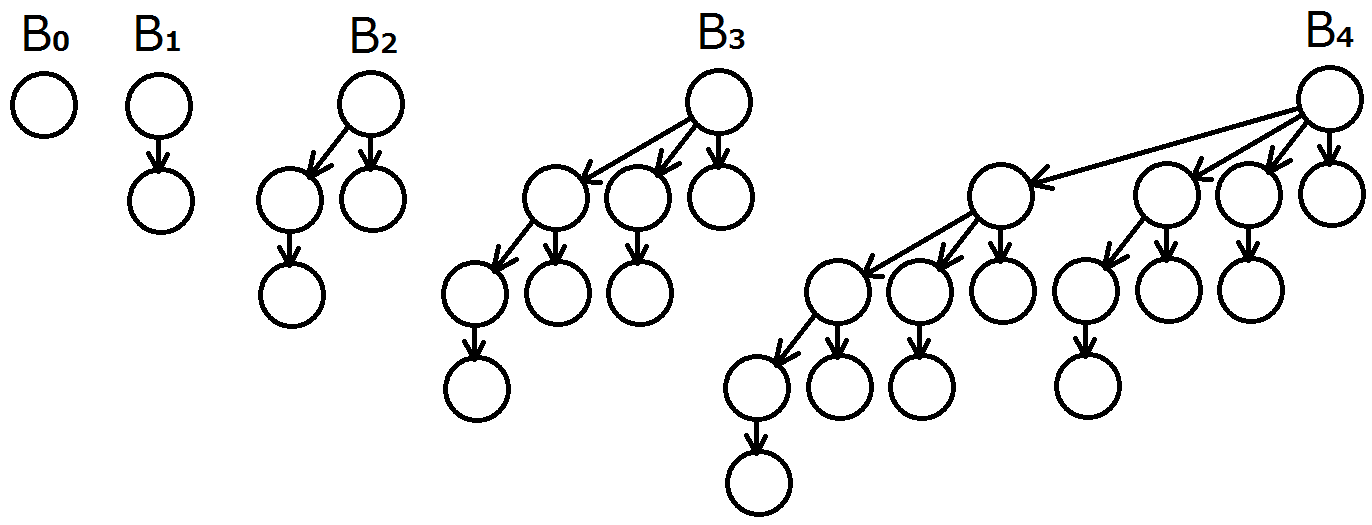
\includegraphics[width=10cm]{image/binomial01.eps}
    }
  \end{exampleblock}
}

\frame{
  \begin{block}{2項木}
    各接点は,親を指すポインタ,最も左の子を指すポインタ,\\
    直接右の兄弟を指すポインタを含んでいる.
  \end{block}
  \begin{exampleblock}{例}
    \center{
      \includegraphics<1>[width=10cm]{image/binomial02.eps}
      \includegraphics<2>[width=3.4cm]{image/binomial03.eps}
    }
  \end{exampleblock}
}

\frame{
  \only<1,2>{
    \begin{block}{2項ヒープ}
      2項ヒープは2項木を小さい順に左から並べた集合として\\
      表現される.
    \end{block}
  }
  \only<3>{
    \frametitle{top}
    \begin{block}{top}
      各2項木の根の中で最大値を探す.$O(\log N)$
    \end{block}
  }
  \begin{exampleblock}{例}
    \center{
      \includegraphics<1>[width=7cm]{image/binomial04.eps}
      \includegraphics<2,3>[width=7cm]{image/binomial05.eps}
    }
  \end{exampleblock}
}

\frame{
  \only<1-6>{
    \frametitle{merge}
    \begin{block}{merge}
      \only<1>{2つの2項ヒープを併合する}
      \only<2>{2項木を小さい順に併合する}
      \only<3-6>{小さい順に同じサイズのヒープがあれば併合する}
    \end{block}
  }
  \only<7>{
    \frametitle{push}
    \begin{block}{push}
      1要素のみからなる二項ヒープをmergeする
    \end{block}
  }
  \begin{exampleblock}{例}
    \center{
      \includegraphics<1>[width=10cm]{image/binomial06.eps}
      \includegraphics<2>[width=10cm]{image/binomial07.eps}
      \includegraphics<3>[width=10cm]{image/binomial08.eps}
      \includegraphics<4>[width=10cm]{image/binomial09.eps}
      \includegraphics<5>[width=10cm]{image/binomial10.eps}
      \includegraphics<6->[width=9cm]{image/binomial11.eps}
    }
  \end{exampleblock}
}

\frame{
  \frametitle{pop}
  \begin{block}{pop}
    \only<1>{最大値の要素を調べる}
    \only<2-3>{最大値を消す}
    \only<4-5>{最大値の要素の子だったものを小さい順に併合する}
    \only<6>{残った2つの二項ヒープをmergeする}
  \end{block}
  \begin{exampleblock}{例}
    \center{
      \includegraphics<1>[width=7cm]{image/binomial12.eps}
      \includegraphics<2>[width=7cm]{image/binomial13.eps}
      \includegraphics<3>[width=7cm]{image/binomial14.eps}
      \includegraphics<4>[width=7cm]{image/binomial15.eps}
      \includegraphics<5-6>[width=7cm]{image/binomial16.eps}
    }
  \end{exampleblock}
}
